\documentclass[a4paper,12pt]{article}
\usepackage[utf8]{inputenc}
\usepackage[francais]{babel}
\usepackage{amsmath}
\usepackage{graphicx}

\title{Projet ECAO Rubiks Cube: Logique Métier\\ - Documentation -}
\author{Bienaimé Pierre, Bonnet Bastien, Chataigner Mathieu,\\ Fresquet Mathieu}

\begin{document}

\maketitle
\tableofcontents
\newpage
\section {Introduction}
Le projet \textit{ECAO Rubiks Cube: Logique Métier} a pour but de développer un programme qui fournit l'ensemble des actions qu'il faut effectuer pour résoudre un Rubik's Cube mélangé.

Ce programme est développé en Java.

Il se place dans le cadre d'un projet du département ASI qui consiste à créer un robot qui résout automatiquement, et de manière autonome, un Rubik's Cube réel.

Ce document vise à expliquer les modalités d'utilisation et le fonctionnement de notre programme. Pour des informations complémentaires, le diagramme de classe orienté Java et la Javadoc de notre projet sont disponibles.

\section{Utilisation du programme}


\subsection{Initialisation des faces}
Pour utiliser ce programme, il faut tout d'abord créer un Rubik's Cube virtuel à partir de ses 6 faces en indiquant la couleur de chaque cubie, en suivant l'ordre du schéma ci-dessous:

\begin{center}
\begin{figure}[!h]
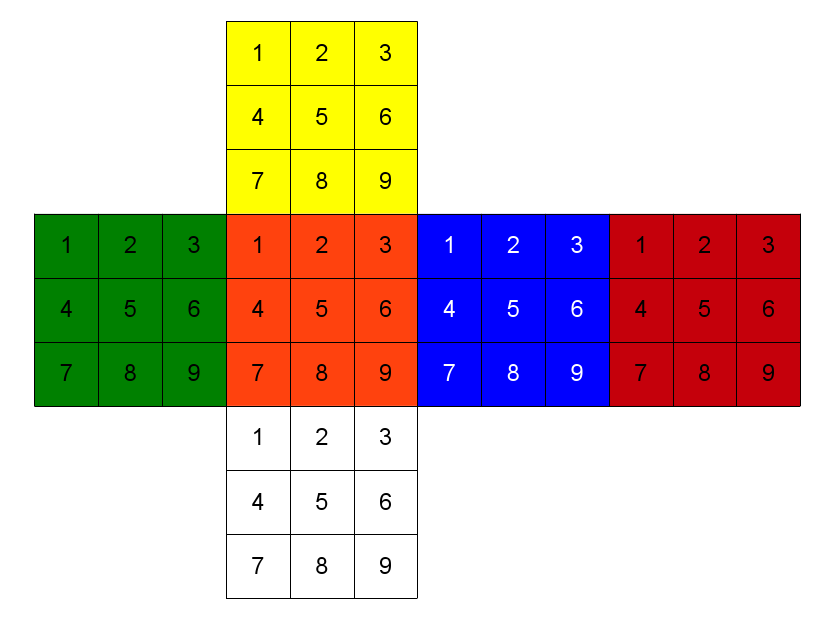
\includegraphics[width=11cm, height=8.5cm]{cube.png}
\caption{ordre de saisie des couleurs des cubies de chaque face du cube}
\end{figure}
\end{center}

Par exemple, voici le code permettant de créer une face à partir de la couleur de ses 9 cubies:

\begin{verbatim}
Face  faceU=new Face(Couleur.JAUNE, Couleur.ROUGE, Couleur.VERT,
Couleur.JAUNE,Couleur.BLANC, Couleur.JAUNE, Couleur.BLEU, 
Couleur.ORANGE, Couleur.BLANC);
\end{verbatim}


\subsection{Initialisation du cube}

A partir de ces 6 faces, on initialise un Cube, comme montré ci dessous:

\begin{verbatim}
Cube leCube=new Cube(faceU, faceD, faceR, faceL, faceF, faceB);
\end{verbatim}

Il est important de respecter l'ordre des faces du cube (c'est à dire U, D, R, L, F puis B). L'objet Cube est ainsi créé.\\

\underline{Remarque:} On peut choisir de créer un cube déjà mélangé, ou de créer un cube résolu, et lui appliqué par la suite un algorithme de mélange.
Voici un exemple d'algorithme visant à mélanger le cube:
\begin{verbatim}
Algorithme algoDeMelange=new Algorithme("D B B R Lp Dp U U Dp U
Fp L L B U R Lp Dp R R Lp B Dp L F D D U Lp Dp Lp Bp U F F");
algoDeMelange.executerSurCube(leCube);
\end{verbatim}

\subsection{Obtention de la solution}

La solution est un Algorithme.
Il existe plusieurs méthodes pour résoudre un Rubik's Cube. Celle que nous avons développé à été baptisée EasyResolution.
Il faut donc instancier un objet EasyResolution à partir d'un Cube.

\begin{verbatim}
EasyResolution er = new EasyResolution(leCube);
\end{verbatim}

Pour obtenir l'algorithme de résolution, il suffit ensuite d'utiliser la méthode trouverSolution.

\begin{verbatim}
Algorithme solution = er.trouverSolution();
\end{verbatim}

Après utilisation de cette methode, \textit{solution} contient l'algorithme permettant de résoudre le cube, et le cube virtuel \textit{leCube} se trouve désormais dans un état résolu.\\

\underline{Remarque:} Des fonctionnalités supplémentaires sont disponibles telles que l'affichage en mode texte d'un Cube, ou de la taille d'un algorithme et de son contenu en mode texte.

\begin{verbatim}
System.out.println("Algorithme de la solution= "+solution.toString());
System.out.println("Taille de la solution= "+solution.taille());
System.out.println("Cube après résolution: "+leCube);
\end{verbatim}

\section{Fonctionnement du programme}

Nous allons maintenant expliquer briévement le fonctionnement de notre programme.\\

\underline{Remarque:} Pensez à consulter le lexique :)\\


Pour obtenir l'algorithme de solution, nous résolvons le cube couronne par couronne.
La couleur d'une face est determinée par la couleur de son cubie central.

Afin de pouvoir nous repérer sur le cube, nous utilisons la classe Position. Nous avons donc créé un repère dont l'origine est le coin formé par les faces L , D  et B.

L'axe des x suit l'arète de la face L et D.

L'axe des y suit l'arète de la face D et B.

L'axe des z suit l'arète de la face L et B.

Les positions ne dépendent pas des cubies, et sont absolues dans le repère.

\subsection{Résolution de la première couronne}

La première étape est la formation d'une croix de la couleur de la face D. Pour cela, on recherche et on place chacun des 4 edges formant la croix.
La deuxième étape est de compléter cette couronne en repérant puis en plaçant les 4 corners.
Pour les corners, par exemple, notre méthodologie est la suivante: on cherche la position du corner qui doit être positionné en 3,3,1. On effectue un algorithme pour l'y placer. Puis on applique le mouvement \textit{y}. On répète ce même procédé 4 fois.

\subsection{Résolution de la deuxième couronne}

Dans cette étape, il s'agit uniquement de placer les 4 edges de la deuxième couronne (Ce qu'on appelle ``Faire les Belges'').
La première couronne étant déja résolue, ces edges se trouvent forcement soit sur la 2eme, soit sur la 3ème couronne. Nous rechercons leur position grace à la méthode repererBelge.
Si un edge se trouve sur la 2ème couronne, mais au mauvais endroit, nous utilisons la méthode debloquerBelge pour le placer sur la 3ème couronne.
Ensuite, nous utilisons 4 fois la méthode placerBelge pour placer chacun des 4 edges en position 3,3,2, en appliquant un mouvement \textit{y} entre chaque étape.

\subsection{Résolution de la troisième couronne}

La résolution de la dernière couronne se divise en deux grandes étapes.

\subsubsection{OLL}
Le but de cette étape est d'orienter tous les cubies de la dernière couronne afin que la face U soit entièrement de sa couleur.
Pour cela, on effectue de nombreux tests afin de déterminer dans quelle configuration le cube se trouve (TypeOrientation), puis on la résoud avec les algorithmes correspondant.

\subsubsection{PLL}
Le but de cette étape est de permuter tous les cubies de la dernière couronne afin de terminer le cube.
Pour cela, on effectue de nombreux tests afin de déterminer dans quelle configuration le cube se trouve (TypePermutation), puis on la résoud avec les algorithmes correspondant.
On divise cette dernière étape en deux: tout d'abord la résolution des 4 corners, puis celle des 4 edges.

\section{Améliorations futures}

Ce programme est fonctionnel mais peut-être optimisé de plusieurs manières:\\

\begin{itemize}
 \item Optimisation de l'algorithme obtenu par la résolution en supprimant ou en combinant les mouvements inutiles, afin de le raccourcir. (Par exemple U U U U peut-être supprimé, et Up Up Up peut-être remplacé par U).
 \item Amélioration de notre EasyResolution en rajoutant des configurations d'OLL et de PLL
 \item Création d'une MediumResolution qui pourrait fusionner la résolution des deux premières couronnes en une seule étape (comme fait par les professionnels en compétition)
 \item Création d'une HardResolution qui pourrait retourner l'algorithme le plus court possible (en théorie, chaque Rubik's Cube peut-être résolu en seulement 25 mouvements environ.)
 \item Création d'une interface graphique permettant de suivre la résolution en temps réel.
\end{itemize}

\section{Lexique: Jargon propre au Rubik's Cube}

Voici un petit lexique du jargon Rubik’s Cube qui vous permettra de
mieux appréhender tous les termes que nous utilisons.\\

\textbf{Cubie }: Une des 27 pièces composant le cube (12 edges, 8 corners, 6
centers et 1 core).\\

\textbf{F2L :} First Two Layers, l’étape qui consiste en la résolution des deux
premières couronnes du Rubik’s Cube.\\

\textbf{OLL :} Orientation Last Layer, l’étape qui permet de résoudre l’orientation de la dernière couronne du Rubik’s Cube.\\

\textbf{PLL :} Permutation Last Layer, l’étape qui permet de résoudre les permutations des cubies de la dernière couronne. C’est la dernière étape de la résolution d’un cube.\\

\textbf{Algorithme :} Suite de mouvements élementaires qui modifie le cube. En général, un algorithme permet de passer d'une étape de la résolution à l'étape suivante.\\

\textbf{Mouvement élementaire :} Rotation d’un quart de tour d’une des tranches du Rubik’s Cube, dans le sens des aiguilles d’une montre : U,D,L,R,F,B
respectivement Up, Down, Left, Right, Front, Back. On rajoute un \textit{p} signifiant \textit{prime} pour indiquer que le mouvement s'effectue dans le sens inverse des aiguilles d'une montre. (par exemple Up, Rp, Lp).
Le mouvement \textit{y} correspond à la rotation du cube entier dans le sens du mouvement U. Le mouvement \textit{x} correspond à la rotation du cube entier dans le sens du mouvement R.\\


Pour toute question ou remarque, n'hesitez pas à nous contacter par e-mail:

pierre.bienaime@insa-rouen.fr

bastien.bonnet@insa-rouen.fr

mathieu.chataigner@insa-rouen.fr

mathieu.fresquet@insa-rouen.fr

\end{document}
